% !TEX encoding = UTF-8 Unicode
\RequirePackage{fix-cm}
\documentclass[a4paper,10pt,UTF8]{paper}
%\documentclass[a4paper,10pt,UTF8]{ctexart}

\usepackage[english]{babel}
\usepackage{fancyhdr,array,lastpage,amsmath,mathtools,enumitem,graphicx,multirow,tocbibind,longtable,makecell,varwidth,titlesec,bm,booktabs,comment}
\usepackage{enumitem}
\usepackage{hyperref}
\hypersetup{hidelinks}
%\setCJKmainfont[BoldFont=Heiti SC Medium]{Songti SC Light}
%\setCJKsansfont{Heiti SC}

\usepackage[left=2.54cm,right=2.54cm,top=2.54cm,bottom=2.54cm]{geometry}
\usepackage[font=footnotesize,labelfont=bf]{caption}
\usepackage{tikz,flowchart}
\usepackage{ctex}
\usetikzlibrary{shapes,shapes.geometric,arrows,matrix,calc}
\usetikzlibrary{circuits.logic}
% \usetikzlibrary{circuits.logic.custom}
\usetikzlibrary{circuits.logic.IEC}
\usetikzlibrary{shadows}
\usepackage{listings}
\usepackage[Q=yes]{examplep}
\usepackage{fancyhdr}
\usepackage{alphalph}
\usepackage{indentfirst}

\newenvironment{sol}
  {\par\vspace{2mm}\noindent{\bf Solution}. }

\lstset{escapeinside=``, breaklines=true, frame=none, extendedchars=false, basicstyle=\ttfamily, showstringspaces=false}


\setlength{\parindent}{2em}
\setlength{\parskip}{1.5ex plus 0.5ex minus 0.2ex}
\linespread{1.1}

\bibliographystyle{plain}

\numberwithin{equation}{section}
\numberwithin{figure}{section}

\usepackage{karnaugh}
\usepackage{circuitikz}


\setcounter{secnumdepth}{3}
\setcounter{tocdepth}{3}

\title{华东师范大学计算机科学技术系上机实验报告}

\begin{document}
\pagestyle{fancy}
\chead{\small\color{gray}华东师范大学计算机科学技术系上机实验报告}
\lhead{}
\rhead{}
\makeatletter
\def\headrule{{\if@fancyplain\let\headrulewidth\plainheadrulewidth\fi%
\color{gray}\hrule\@height 0.2pt\@width\headwidth}
  \vspace{6mm}}
\makeatother

\newcommand{\HRule}{\rule{\linewidth}{1mm}}
\newcommand{\dai}{\textbf{Dais-CMX16$^+$}}

{\center {\huge \bfseries \LARGE{华东师范大学计算机科学技术系上机实验报告}} \\ [0.8cm]

\small{
  \begin{minipage}[t]{.32\linewidth}
    \textbf{课程名称:}计算机组成与结构实践\\
    \textbf{指导教师:}金健\\
    \textbf{上机实践名称:} 十六位机运算器实验\\
    \textbf{实践编号:}实验 2
  \end{minipage}
  \begin{minipage}[t]{.32\linewidth}
    \textbf{年级:}17 级\\
    \textbf{姓名:}朱桐\\
    \textbf{学号:}10175102111\\
    \textbf{组号:}A
  \end{minipage} 
  \begin{minipage}[t]{.32\linewidth}
    \textbf{上机实践成绩:} \\
    \textbf{创新实践成绩:} \\
    \textbf{上机实践日期:}2019/09/27\\
    \textbf{上机实践时间:}2 学时\\
  \end{minipage}
}
\HRule \\[0.5cm]
}
\section{实验目的}

\begin{enumerate}
    \item 掌握十六位机字与字节运算的数据传输格式
    \item 验证ALU及标志位控制的组合功能
    \item 熟悉ALU运算控制位的运用
\end{enumerate}

\section{实验设备}

\dai 设备一台

\section{实验内容}

使用手动搭接的方法,实现ALU的输入并且完成各种运算输出

\section{实验原理}

\subsection{数据通路}

实验中所用的运算器数据通路如图 \ref{fig:datapath} 所示。ALU 运算器由CPLD 描述。运算器的输出经
过2 片74LS245 三态门与数据总线相连,2 个运算寄存器AX、BX 的数据输入端分别由4 个
74LS574 锁存器锁存,锁存器的输入端与数据总线相连,准双向I/O 输入输出端口用来给出参与
运算的数据,经2 片74LS245 三态门与数据总线相连。


\begin{figure}[h]
  \centering
  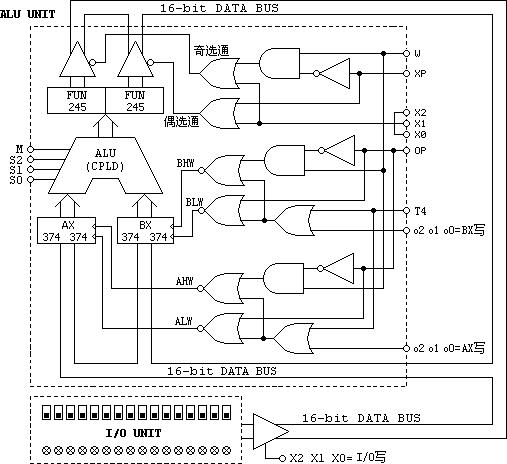
\includegraphics[width=0.7\textwidth]{1.jpg}
  \caption{运算器数据通路}
  \label{fig:datapath}
\end{figure}

\subsection{运算器功能码}

运算器功能吗如图 \ref{fig:funcode} 所示。我们通过设置不同的功能码完成各种不同的运算

\begin{figure}[h]
  \centering
  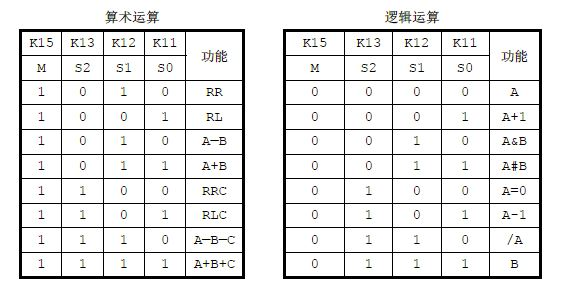
\includegraphics[width=0.7\textwidth]{2.JPG}
  \caption{运算器功能码}
  \label{fig:funcode}
\end{figure}


\section{实验步骤}

\subsection{ ALU 输入 }

从 I/O 到总线的输入已经在上一次实验了解过了,这里与输出到通用寄存器组 CX 开启 RWX 不同的是,我们开启开关 AWX 和 BWX 控制总线到 ALU 的输入寄存器

% \subsection{运算影响标志位/标志位带入运算 }

% \begin{itemize}
%   \item 设置 $M=1$
%   \item 进行算术运算
%   \item 运算影响标志位 
%   \item 只要运算类型是带标志位(CY),则将带入运算
  
% \end{itemize}

\subsection{算术运算}

\subsubsection{字运算}

\begin{itemize}
  \item 令 $MS_2S_1S_0=K{15}K{13}K{12}K_{11}=1011$,$FUN$ 及总线单元显示 $AX+BX$ 的结果
  \item 令 $MS_2S_1S_0=K{15}K{13}K{12}K_{11}=1010$,FUN 及总线单元显示 AX-BX 的结果

\end{itemize}

\subsubsection{字节运算}

我们通过控制 $XP,W$ 来控制 $AX, BX$ 的有效位来进行字节运算


\subsection{逻辑运算}

\subsubsection{字运算}

\begin{itemize}
  \item 令 $MS_2S_1S_0=K{15}K{13}K{12}K_{11}=0010$,$FUN$ 及总线单元显示 $AX \& BX$ 的结果
  \item 令 $MS_2S_1S_0=K{15}K{13}K{12}K_{11}=0011$,$FUN$ 及总线单元显示 $AX | BX$ 的结果
\end{itemize}

\subsubsection{字节运算}

我们通过控制 $XP,W$ 来控制 $AX, BX$ 的有效位来进行字节运算

\subsection{带进位运算}

\subsubsection{进位控制}

\begin{itemize}
  \item 按 [返回] 初始化进位标志 $CY=0$
  \item 设置 $CN=1$,改变 $XP,W$
  \item 按单拍
\end{itemize}

其中进位控制编码如图\ref{fig:cycode}所示


\begin{figure}[h]
  \centering
  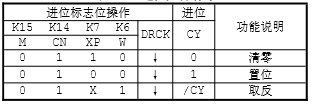
\includegraphics[width=0.7\textwidth]{3.PNG}
  \caption{进位控制编码}
  \label{fig:cycode}
\end{figure}

\subsubsection{进位运算}

\begin{itemize}
  \item $X_2X_1X_0=001,XPW=11$
  \item $M=1 S_2S_1=11$
  \item $S0=0$ 为减法,否则为加法
\end{itemize}


\subsection{零标志}

进行运算后,$Z$ 标志按钮会随着运算结果变化而变化

\subsection{ ALU 到 BUS 和 BUS 到 IO}


我们通过 $X_2X_1X_0 = 001$ 来设置总线的输入设备位 ALU,和上次实验一样,设置 $IOW = 1$ 并且给 $IRCK$ 一个脉冲,便可完成总线到 I/O 的输出。


\section{调试过程、结果与分析}

\subsection{实验要求}

假设CY原来有值,在进行带进位加法时,加法结果可能会产生新的进位,也可能不产 生。请分析这种情况,设计实验验证各种情况下加法完成后CY的值

\subsection{分析}

我们已经知道了手动控制 $CY$,和控制 $CY$ 是否带入运算的方法,且 $CY$ 于加法表示加法进位,减法表示减法进位。因此我们可以推断出

\begin{itemize}
  \item 加法带进位运算 $MS_2S_1S_0=1111$, 若原来 $AX=0001,BX=0003,CY=1$, 则结果 $DBUS=FUN=0005$,不产生新的进位
  \item 加法带进位运算 $MS_2S_1S_0=1111$,若原来 $AX=000F,BX=000F,CY=1$, 则结果 $DBUS=FUN=000F$,产生新的进位
  \item 减法带进位运算 $MS_2S_1S_0=1110$,若原来 $AX=000F,BX=000F,CY=1$, 则结果 $DBUS=FUN=000F$,产生新的进位
  \item 减法带进位运算 $MS_2S_1S_0=1110$,若原来 $AX=000F,BX=000E,CY=1$, 则结果 $DBUS=FUN=0000$,不产生新的进位
\end{itemize}

\section{总结}

\section{附件}

\end{document}
